\documentclass[../../../../../../../dd.tex]{subfiles}

\begin{document}

	\subsubsection{Profile Manager}
		This component have to check if a registration or a login request is legal or not and if it is, then the relative function of the Database Manager has to be called.
		\begin{itemize}
			\item \textbf{Registration Manager:} This sub-component is in charge to accept registration requests from IO Manager and Facebook API Manager, check the credentials using the Credential Checker and then if it's the case register a new user using the functions provided by the Database Manager.

			\item \textbf{Login Manager:} This sub-component is in charge to accept login requests from IO Manager and Facebook API Manager, check the credentials using the Credential Checker and then if it's the case set a user as logged in using the functions provided by the Database Manager.

			\item \textbf{Profile Modifier:} This sub-component is in charge to accept profile modification requests from the IO Manager, check the new credentials and, if it's the case, change the profile credentials using the functions provided by the Database Manager.

			\item \textbf{Profile Viewer:} This sub-component is in charge to provide to the IO Manager information about an user.

			\item \textbf{Credential Checker:} This sub-component is in charge to check the credentials provided by the others sub-components. Here are implemented all the rules about the acceptance of users credentials (like password composition policy etc...).
		\end{itemize}

		\begin{figure}[H]
				\centering
				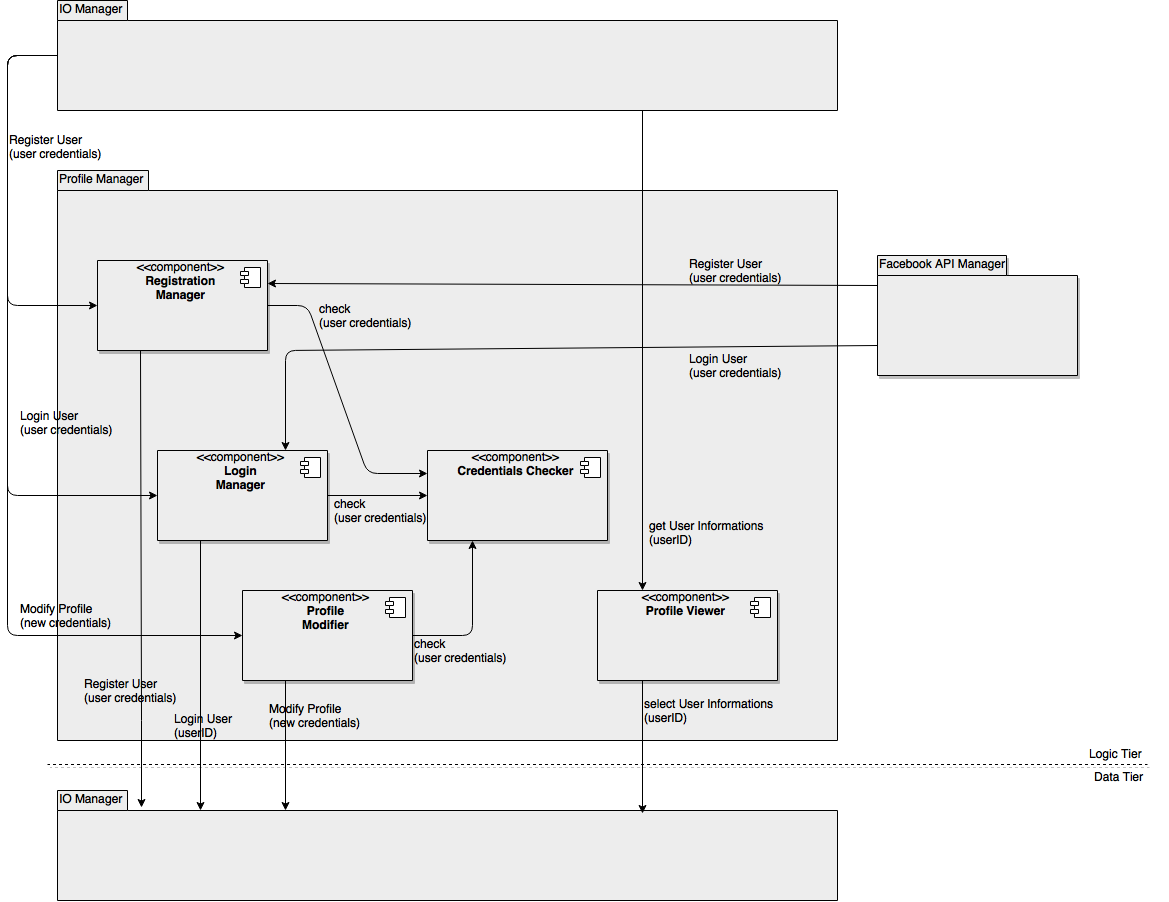
\includegraphics[width=\textwidth, scale=0.5]{../images/ProfileManager.png}
			\caption{Profile Manager Structure}\label{fig:ProfileManager}
		\end{figure}
		
\end{document}